
\def\slidemode{
  \documentclass[fleqn,aspectratio=169]{beamer}
\usepackage{pgfpages}
}
\def\handoutmode{
  \documentclass[handout,fleqn,aspectratio=169]{beamer}
\usepackage{pgfpages}
\pgfpagesuselayout{resize to}[a4paper,landscape,border shrink=5mm]
}


%\def\pdfmode{handoutmode}
\def\pdfmode{slidemode}

\csname\pdfmode\endcsname

\mode<presentation>
{
  \usetheme{default}
  \usecolortheme{default}
  \usefonttheme{default}
  \setbeamertemplate{navigation symbols}{}
  \setbeamertemplate{caption}[numbered]
  \setbeamertemplate{footline}[frame number]  % or "page number"
  \setbeamercolor{frametitle}{fg=white}
  \setbeamercolor{footline}{fg=black}
}

\usepackage[english]{babel}
%\usepackage[utf8x]{inputenc}
\usepackage{tikz}
\usepackage{courier}
\usepackage{array}
\usepackage{bold-extra}
%\usepackage{minted}
%\usepackage[thicklines]{cancel}
%\usepackage{fancyvrb}
\usepackage{kotex}
\usepackage{paralist}
\usepackage{collectbox}
\usepackage{amsmath}
\usepackage{mathtools}
\usepackage{nccmath}
\usepackage{bm}
\usepackage{booktabs}
\usepackage{tcolorbox}
\usepackage[absolute,overlay]{textpos}

\xdefinecolor{dianablue}{rgb}{0.18,0.24,0.31}
\xdefinecolor{darkblue}{rgb}{0.1,0.1,0.7}
\xdefinecolor{darkgreen}{rgb}{0,0.5,0}
\xdefinecolor{darkgrey}{rgb}{0.35,0.35,0.35}
\xdefinecolor{darkorange}{rgb}{0.8,0.5,0}
\xdefinecolor{darkred}{rgb}{0.7,0,0}
\definecolor{darkgreen}{rgb}{0,0.6,0}
\definecolor{mauve}{rgb}{0.58,0,0.82}



\title[]{Lecture 4: Random Variable, Part II}
\author{Yi, Yung (이융)}
\institute{EE210: Probability and Introductory Random Processes\\ KAIST EE}
\date{\today}





%%%%%%%%%%%% real, integer notation
\newcommand{\real}{{\mathbb R}}
\newcommand{\integer}{{\mathbb Z}}

%%% set, vector, matrix
\newcommand{\set}[1]{\ensuremath{\mathcal #1}}
\renewcommand{\vec}[1]{\bm{#1}}
\newcommand{\mat}[1]{\bm{#1}}


%%% big parenthesis
\def\Bl{\Bigl}
\def\Br{\Bigr}
\def\lf{\left}
\def\ri{\right}


%%% floor notations
\newcommand{\lfl}{{\lfloor}}
\newcommand{\rfl}{{\rfloor}}
\newcommand{\floor}[1]{{\lfloor #1 \rfloor}}

%%% gradient
\newcommand{\grad}[1]{\nabla #1}

%%% definition
\newcommand{\eqdef}{\ensuremath{\triangleq}}
%%% imply
\newcommand{\imp}{\Longrightarrow}



\newcommand{\separator}{
%  \begin{center}
    \par\noindent\rule{\columnwidth}{0.3mm}
%  \end{center}
}

\newcommand{\mynote}[1]{{\it \color{red} [#1]}}







%%% equation alignment
\newcommand{\aleq}[1]{\begin{align*}#1\end{align*}}

%%%%%%%%%%%%%%%% colored emphasized font, blanked words

\newcommand{\empr}[1]{{\color{red}\emph{#1}}}
\newcommand{\empb}[1]{{\color{blue}\emph{#1}}}

%normal colored text
\newcommand{\redf}[1]{{\color{red} #1}}
\newcommand{\yellowf}[1]{{\color{yellow} #1}}
\newcommand{\bluef}[1]{{\color{blue} #1}}
\newcommand{\grayf}[1]{{\color{gray} #1}}
\newcommand{\magenf}[1]{{\color{magenta} #1}}
\newcommand{\greenf}[1]{{\color{green} #1}}
\newcommand{\cyanf}[1]{{\color{cyan} #1}}
\newcommand{\orangef}[1]{{\color{orange} #1}}


\newcommand{\blk}[1]{\underline{\mbox{\hspace{#1}}}}


\newcommand{\redblk}[1]{\framebox{\color{red} #1}}
\newcommand{\redblank}[2]{\framebox{\onslide<#1->{\color{red} #2}}}
\newcommand{\blueblk}[1]{\framebox{\color{blue} #1}}
\newcommand{\blueblank}[2]{\framebox{\onslide<#1->{\color{blue} #2}}}



\makeatletter
\newcommand{\mybox}{%
    \collectbox{%
        \setlength{\fboxsep}{1pt}%
        \fbox{\BOXCONTENT}%
    }%
}
\makeatother

\makeatletter
\newcommand{\lecturemark}{%
    \collectbox{%
        \setlength{\fboxsep}{1pt}%
        \fcolorbox{red}{yellow}{\BOXCONTENT}%
    }%
}
\makeatother

\usepackage{tcolorbox}
\newcommand{\mycolorbox}[1]{
\begin{tcolorbox}[colback=red!5!white,colframe=red!75!black]
#1
\end{tcolorbox}
}

%%%% figure inclusion
\newcommand{\mypic}[2]{
\begin{center}
\includegraphics[width=#1\textwidth]{#2}
\end{center}
}

\newcommand{\myinlinepic}[2]{
\makebox[0cm][r]{\raisebox{-4ex}{\includegraphics[height=#1]{#2}}}
}


%%%% itemized and enumerated list
\newcommand{\bci}{\begin{compactitem}}
\newcommand{\eci}{\end{compactitem}}
\newcommand{\bce}{\begin{compactenum}}
\newcommand{\ece}{\end{compactenum}}


%%%% making 0.5/0.5 two columns
%%%% how to use: first number: length of separation bar
% \mytwocols{0.6}
% {
% contents in the left column
% }
% {
% contents in the right column
% }
%%%%
\newcommand{\mytwocols}[3]{
\begin{columns}[T] \column{.499\textwidth} #2 \column{.001\textwidth} \rule{.3mm}{{#1}\textheight} \column{.499\textwidth} #3 \end{columns}}

\newcommand{\mythreecols}[4]{
\begin{columns}[T] \column{.31\textwidth} #2 \column{.001\textwidth} \rule{.3mm}{{#1}\textheight} \column{.31\textwidth} #3 \column{.001\textwidth} \rule{.3mm}{{#1}\textheight} \column{.31\textwidth} #4  \end{columns}}

\newcommand{\mysmalltwocols}[3]{
\begin{columns}[T] \column{.4\textwidth} #2 \column{.001\textwidth} \rule{.3mm}{{#1}\textheight} \column{.4\textwidth} #3 \end{columns}}

%%%% making two columns with customized ratios
%%%% how to use:
%first parameter: length of separation bar
%second parameter: ratio of left column
%third parameter: ratio of right column
% \mytwocols{0.6}{0.7}{0.29}
% {
% contents in the left column
% }
% {
% contents in the right column
% }
%%%%
\newcommand{\myvartwocols}[5]{
\begin{columns}[T] \column{#2\textwidth} {#4} \column{.01\textwidth} \rule{.3mm}{{#1}\textheight} \column{#3\textwidth} {#5} \end{columns}}

%%% making my block in beamer
%%% first parameter: title of block
%%% second parameter: contents of block
\newcommand{\myblock}[2]{
\begin{block}{#1} {#2}  \end{block}}

%%% independence notation
\newcommand{\indep}{\perp \!\!\! \perp}

%%%% probability with different shapes (parenthesis or bracket) and different sizes
%%% `i' enables us to insert the subscript to the probability
\newcommand{\bprob}[1]{\mathbb{P}\Bl[ #1 \Br]}
\newcommand{\prob}[1]{\mathbb{P}[ #1 ]}
\newcommand{\cbprob}[1]{\mathbb{P}\Bl( #1 \Br)}
\newcommand{\cprob}[1]{\mathbb{P}( #1 )}
\newcommand{\probi}[2]{\mathbb{P}_{#1}[ #2 ]}
\newcommand{\bprobi}[2]{\mathbb{P}_{#1}\Bl[ #2 \Br]}
\newcommand{\cprobi}[2]{\mathbb{P}_{#1}( #2 )}
\newcommand{\cbprobi}[2]{\mathbb{P}_{#1}\Bl( #2 \Br)}

%%%% expectation with different shapes (parenthesis or bracket) and different sizes
%%% `i' enables us to insert the subscript to the expectation
\newcommand{\expect}[1]{\mathbb{E}[ #1 ]}
\newcommand{\cexpect}[1]{\mathbb{E}( #1 )}
\newcommand{\bexpect}[1]{\mathbb{E}\Bl[ #1 \Br]}
\newcommand{\cbexpect}[1]{\mathbb{E}\Bl( #1 \Br)}
\newcommand{\bbexpect}[1]{\mathbb{E}\lf[ #1 \ri]}
\newcommand{\expecti}[2]{\mathbb{E}_{#1}[ #2 ]}
\newcommand{\bexpecti}[2]{\mathbb{E}_{#1}\Bl[ #2 \Br]}
\newcommand{\bbexpecti}[2]{\mathbb{E}_{#1}\lf[ #2 \ri]}

%%%% variance
\newcommand{\var}[1]{\text{var}[ #1 ]}
\newcommand{\bvar}[1]{\text{var}\Bl[ #1 \Br]}
\newcommand{\cvar}[1]{\text{var}( #1 )}
\newcommand{\cbvar}[1]{\text{var}\Bl( #1 \Br)}

%%%% covariance
\newcommand{\cov}[1]{\text{cov}( #1 )}
\newcommand{\bcov}[1]{\text{cov}\Bl( #1 \Br)}

%%% Popular pmf, pdf notation to avoid long typing
\newcommand{\px}{\ensuremath{p_X(x)}}
\newcommand{\py}{\ensuremath{p_Y(y)}}
\newcommand{\pz}{\ensuremath{p_Z(z)}}
\newcommand{\pxA}{\ensuremath{p_{X|A}(x)}}
\newcommand{\pyA}{\ensuremath{p_{Y|A}(y)}}
\newcommand{\pzA}{\ensuremath{p_{Z|A}(z)}}
\newcommand{\pxy}{\ensuremath{p_{X,Y}(x,y)}}
\newcommand{\pxcy}{\ensuremath{p_{X|Y}(x|y)}}
\newcommand{\pycx}{\ensuremath{p_{Y|X}(y|x)}}

\newcommand{\fx}{\ensuremath{f_X(x)}}
\newcommand{\Fx}{\ensuremath{F_X(x)}}
\newcommand{\fy}{\ensuremath{f_Y(y)}}
\newcommand{\Fy}{\ensuremath{F_Y(y)}}
\newcommand{\fz}{\ensuremath{f_Z(z)}}
\newcommand{\Fz}{\ensuremath{F_Z(z)}}
\newcommand{\fxA}{\ensuremath{f_{X|A}(x)}}
\newcommand{\fyA}{\ensuremath{f_{Y|A}(y)}}
\newcommand{\fzA}{\ensuremath{f_{Z|A}(z)}}
\newcommand{\fxy}{\ensuremath{f_{X,Y}(x,y)}}
\newcommand{\Fxy}{\ensuremath{F_{X,Y}(x,y)}}
\newcommand{\fxcy}{\ensuremath{f_{X|Y}(x|y)}}
\newcommand{\fycx}{\ensuremath{f_{Y|X}(y|x)}}

\newcommand{\fth}{\ensuremath{f_\Theta(\theta)}}
\newcommand{\fxcth}{\ensuremath{f_{X|\Theta}(x|\theta)}}
\newcommand{\fthcx}{\ensuremath{f_{\Theta|X}(\theta|x)}}

\newcommand{\pkcth}{\ensuremath{p_{X|\Theta}(k|\theta)}}
\newcommand{\fthck}{\ensuremath{f_{\Theta|X}(\theta|k)}}


%%%% indicator
\newcommand{\indi}[1]{\mathbf{1}_{ #1 }}

%%%% exponential rv.
\newcommand{\elambdax}{\ensuremath{e^{-\lambda x}}}

%%%% normal  rv.
\newcommand{\stdnormal}{\ensuremath{\frac{1}{\sqrt{2\pi}} e^{-x^2/2}}}
\newcommand{\gennormal}{\ensuremath{\frac{1}{\sigma\sqrt{2\pi}} e^{-(x-\mu)^2/2}}}

%%%%%% estimator, estimate
\newcommand{\hth}{\ensuremath{\hat{\theta}}}
\newcommand{\hTH}{\ensuremath{\hat{\Theta}}}
\newcommand{\MAP}{\ensuremath{\text{MAP}}}
\newcommand{\LMS}{\ensuremath{\text{LMS}}}
\newcommand{\LLMS}{\ensuremath{\text{L}}}
\newcommand{\ML}{\ensuremath{\text{ML}}}

%%%% colored text
\newcommand{\red}[1]{\color{red}#1}
\newcommand{\cyan}[1]{\color{cyan}#1}
\newcommand{\magenta}[1]{\color{magenta}#1}
\newcommand{\blue}[1]{\color{blue}#1}
\newcommand{\green}[1]{\color{green}#1}
\newcommand{\white}[1]{\color{white}#1}

\newcommand{\defi}{{\color{red} Definition.} }
\newcommand{\proff}{{\color{red} Proof.} }
\newcommand{\exam}{{\color{red} Example.} }
\newcommand{\question}{{\color{red} Question.} }
\newcommand{\thm}{{\color{red} Theorem.} }
\newcommand{\background}{{\color{red} Background.} }
\newcommand{\msg}{{\color{red} Message.} }

\newcommand{\bern}[1]{\ensuremath{\text{Bern}(#1)} }
\newcommand{\bp}[1]{\ensuremath{\text{BP}(#1)} }
\newcommand{\poisson}[1]{\ensuremath{\text{Poisson}(#1)} }
\newcommand{\pp}[1]{\ensuremath{\text{PP}(#1)} }


%%%%%%%%%%%%%%%%%%%%%%% old macros that you can ignore %%%%%%%%%%%%%%%%%%%%%%%%

% \def\un{\underline}
% \def\ov{\overline}


% \newcommand{\beq}{\begin{eqnarray*}}
% \newcommand{\eeq}{\end{eqnarray*}}
% \newcommand{\beqn}{\begin{eqnarray}}
% \newcommand{\eeqn}{\end{eqnarray}}
% \newcommand{\bemn}{\begin{multiline}}
% \newcommand{\eemn}{\end{multiline}}
% \newcommand{\beal}{\begin{align}}
% \newcommand{\eeal}{\end{align}}
% \newcommand{\beas}{\begin{align*}}
% \newcommand{\eeas}{\end{align*}}



% \newcommand{\bd}{\begin{displaymath}}
% \newcommand{\ed}{\end{displaymath}}
% \newcommand{\bee}{\begin{equation}}
% \newcommand{\eee}{\end{equation}}


% \newcommand{\vs}{\vspace{0.2in}}
% \newcommand{\hs}{\hspace{0.5in}}
% \newcommand{\el}{\end{flushleft}}
% \newcommand{\bl}{\begin{flushleft}}
% \newcommand{\bc}{\begin{center}}
% \newcommand{\ec}{\end{center}}
% \newcommand{\remove}[1]{}

% \newtheorem{theorem}{Theorem}
% \newtheorem{corollary}{Corollary}
% \newtheorem{prop}{Proposition}
% \newtheorem{lemma}{Lemma}
% \newtheorem{defi}{Definition}
% \newtheorem{assum}{Assumption}
% \newtheorem{example}{Example}
% \newtheorem{property}{Property}
% \newtheorem{remark}{Remark}

% \newcommand{\separator}{
%   \begin{center}
%     \rule{\columnwidth}{0.3mm}
%   \end{center}
% }

% \newenvironment{separation}
% { \vspace{-0.3cm}
%   \separator
%   \vspace{-0.25cm}
% }
% {
%   \vspace{-0.5cm}
%   \separator
%   \vspace{-0.15cm}
% }

% \def\A{\mathcal A}
% \def\oA{\overline{\mathcal A}}
% \def\S{\mathcal S}
% \def\D{\mathcal D}
% \def\eff{{\rm Eff}}
% \def\bD{\bm{D}}
% \def\cU{{\cal U}}
% \def\bbs{{\mathbb{s}}}
% \def\bbS{{\mathbb{S} }}
% \def\cM{{\cal M}}
% \def\bV{{\bm{V}}}
% \def\cH{{\cal H}}
% \def\ch{{\cal h}}
% \def\cR{{\cal R}}
% \def\cV{{\cal V}}
% \def\cA{{\cal A}}
% \def\cX{{\cal X}}
% \def\cN{{\cal N}}
% \def\cJ{{\cal J}}
% \def\cK{{\cal K}}
% \def\cL{{\cal L}}
% \def\cI{{\cal I}}
% \def\cY{{\cal Y}}
% \def\cZ{{\cal Z}}
% \def\cC{{\cal C}}
% \def\cR{{\cal R}}
% \def\id{{\rm Id}}
% \def\st{{\rm st}}
% \def\cF{{\cal F}}
% \def\bz{{\bm z}}
% \def\cG{{\cal G}}
% \def\N{\mathbb{N}}
% \def\bbh{\mathbb{h}}
% \def\bbH{\mathbb{H}}
% \def\bbi{\mathbb{i}}
% \def\bbI{\mathbb{I}}
% \def\R{\mathbb{R}}
% \def\bbR{\mathbb{R}}
% \def\bbr{\mathbb{r}}
% \def\cB{{\cal B}}
% \def\cP{{\cal P}}
% \def\cS{{\cal S}}
% \def\bW{{\bm W}}
% \def\bc{{\bm c}}

% %\def\and{\quad\mbox{and}\quad}
% \def\ind{{\bf 1}}


% \def\bmg{{\bm{\gamma}}}
% \def\bmr{{\bm{\rho}}}
% \def\bmq{{\bm{q}}}
% \def\bmt{{\bm{\tau}}}
% \def\bmn{{\bm{n}}}
% \def\bmcapn{{\bm{N}}}
% \def\bmrho{{\bm{\rho}}}

% \def\igam{\underline{\gamma}(\lambda)}
% \def\sgam{\overline{\gamma}(\lambda)}
% \def\ovt{\overline{\theta}}
% \def\ovT{\overline{\Theta}}
% \def\PP{{\mathrm P}}
% \def\EE{{\mathrm E}}
% \def\iskip{{\vskip -0.4cm}}
% \def\siskip{{\vskip -0.2cm}}

% \def\bp{\noindent{\it Proof.}\ }
% \def\ep{\hfill $\Box$}


\begin{document}

%itemshape
\setbeamertemplate{itemize item}{\scriptsize\raise1.25pt\hbox{\donotcoloroutermaths$\bullet$}}
\setbeamertemplate{itemize subitem}{\tiny\raise1.5pt\hbox{\donotcoloroutermaths$\circ$}}
\setbeamertemplate{itemize subsubitem}{\tiny\raise1.5pt\hbox{\donotcoloroutermaths$\blacktriangleright$}}
%default value for spacing
\plitemsep 0.1in
\pltopsep 0.03in
\setlength{\parskip}{0.15in}
%\setlength{\parindent}{-0.5in}
\setlength{\abovedisplayskip}{0.07in}
\setlength{\mathindent}{0cm}
\setbeamertemplate{frametitle continuation}{[\insertcontinuationcount]}

\setlength{\leftmargini}{0.5cm}
\setlength{\leftmarginii}{0.5cm}

\setlength{\fboxrule}{0.05pt}
\setlength{\fboxsep}{5pt}


\begin{frame}
  \titlepage
\end{frame}


% START START START START START START START START START START START START START

% %%%%%%%%%%%%%%%%%%%%%%%%%%%%%%%%%%%%%%%%%%%%%%%%%%%%%%

\begin{frame}{Roadmap}


\plitemsep 0.1in
\bce[(1)]
\item Continuous Random Variable and PDF (Probability Density Function)

\item CDF (Cumulative Distribution Function)

\item Exponential RVs

\item Gaussian (Normal) RVs

\item Continuous RVs: Joint, Conditioning, and Independence

\item Bayes' rule for RVs

\ece
\end{frame}

% %%%%%%%%%%%%%%%%%%%%%%%%%%%%%%%%%%%%%%%%%%%%%%%%%%%%%%
\section{L4(1)}
\begin{frame}{Roadmap}

\plitemsep 0.1in
\bce[(1)]
\item \redf{Continuous Random Variable and PDF (Probability Density Function)}

\item \grayf{CDF (Cumulative Distribution Function)

\item Exponential RVs

\item Gaussian (Normal) RVs

\item Continuous RVs: Joint, Conditioning, and Independence

\item Bayes' rule for RVs}

\ece
\end{frame}



%%%%%%%%%%%%%%%%%%%%%%%%%%%%%%%%%%%%%%%%%%%%%%%%%%%%%%
\begin{frame}{Continuous RV and Probability Density Function}
\small

\smallskip

\onslide<2->{- Many cases when random variables have ``continuous values", e.g., velocity of a car}
\onslide<3->{
\mycolorbox
{
A rv $X$ is \redf{continuous} if $\exists$ a function $f_X,$ called \redblk{probability density function (PDF)}, s.t.
\vspace{-0.3cm}
$$
\cprob{X \in B} = \int_B \fx dx, \qquad \text{every subset $B \in \real$}
$$
\vspace{-0.5cm}
}}
\vspace{-0.1cm}
\onslide<4->{- All of the concepts and methods (expectation, PMFs, and conditioning) for discrete rvs have continuous counterparts}
\vspace{-0.2cm}
\mytwocols{0.4}
{
\onslide<5->{
\vspace{-0.3cm}
\mypic{0.55}{L4_pmf_ex.png}
\vspace{-0.3cm}
\plitemsep 0.01in
\bci
\item $\cprob{a \le X \le b} = \sum_{x: a\le x \le b} \px$

\item $\px \ge 0,$ $\sum_{x} \px = 1$
\eci}
}
{
\onslide<6->{
\vspace{-0.2cm}
\mypic{0.65}{L4_pdf_ex.png}

\plitemsep 0.01in
\bci
\item $\cprob{a \le X \le b} = \int_{a}^b \fx dx$

\item $\fx \ge 0,$ $\int_{-\infty}^{\infty} \fx dx= 1$
\eci}
}
\end{frame}

%%%%%%%%%%%%%%%%%%%%%%%%%%%%%%%%%%%%%%%%%%%%%%%%%%%%%%
\begin{frame}{PDF and Examples}


\mytwocols{0.7}
{
\onslide<1->{
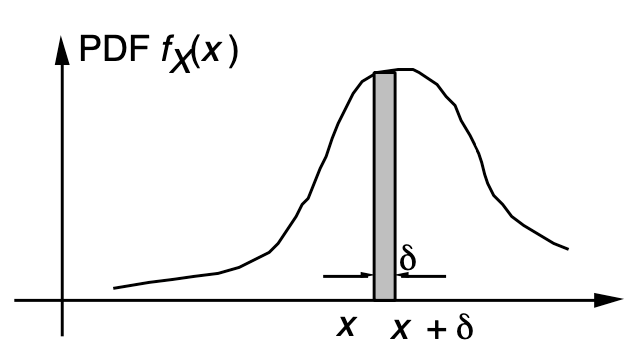
\includegraphics[width=0.65\textwidth]{L4_pdf_delta.png}

\bigskip

\plitemsep 0.1in
\bci
\item $\cprob{a \le X \le a + \delta} \approx$ \redblank{2}{$f_X(a) \cdot \delta$}

\item \onslide<3->{$\cprob{X = a} = 0$}
\eci
}
}
{
Examples

\onslide<4->{
\bigskip

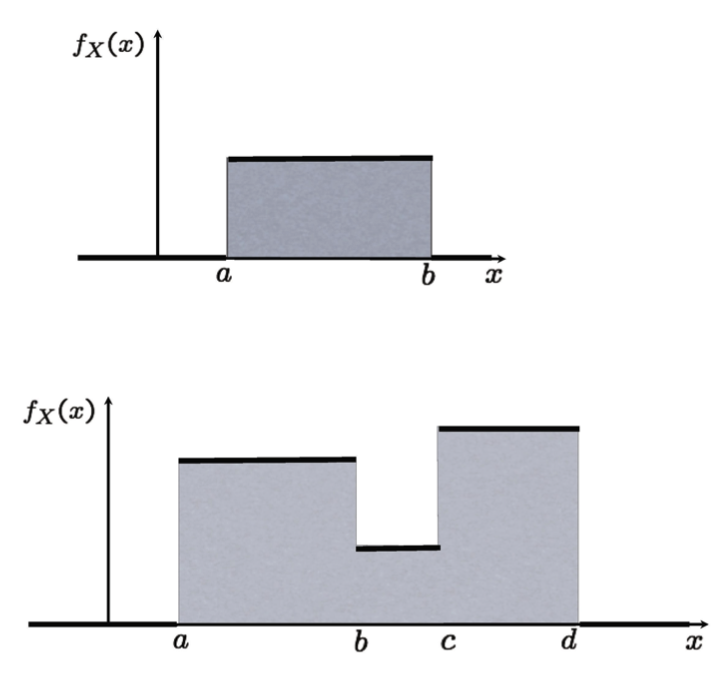
\includegraphics[width=0.8\textwidth]{L4_pdf_uniform_ex.png}
}
}
\end{frame}

%%%%%%%%%%%%%%%%%%%%%%%%%%%%%%%%%%%%%%%%%%%%%%%%%%%%%%
\begin{frame}{Expectation and Variance}


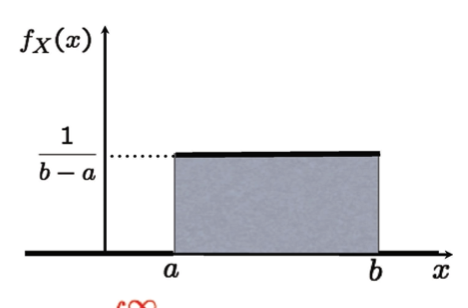
\includegraphics[width=0.3\textwidth]{L4_uniform_ex.png}

\bigskip

\plitemsep 0.1in
\bci
\item $\expect{X} = \int_{-\infty}^{\infty} x \fx dx$ = \onslide<2->{$\int_{a}^{b} \frac{x}{b-a} dx = \frac{1}{b-a}\frac{b^2 - a^2}{2} = \frac{b+a}{2}$}

\item $\expect{X^2} = \int_{-\infty}^{\infty} x^2 \fx dx$ = \onslide<3->{$\int_{a}^{b} \frac{x^2}{b-a} dx = \frac{1}{b-a}\frac{b^3 - a^3}{3} = \frac{a^2 + ab + b^2}{3}$}

\item $\var{X}$ = \onslide<4->{$\frac{a^2 + ab + b^2}{3} - \frac{a^2 + 2ab + b^2}{4}$}
\eci


\end{frame}

% %%%%%%%%%%%%%%%%%%%%%%%%%%%%%%%%%%%%%%%%%%%%%%%%%%%%%%
\section{L4(2)}
\begin{frame}{Roadmap}

\plitemsep 0.1in
\bce[(1)]
\item \grayf{Continuous Random Variable and PDF (Probability Density Function)}

\item \redf{CDF (Cumulative Distribution Function)}

\item \grayf{Exponential RVs

\item Gaussian (Normal) RVs

\item Continuous RVs: Joint, Conditioning, and Independence

\item Bayes' rule for RVs}

\ece
\end{frame}


%%%%%%%%%%%%%%%%%%%%%%%%%%%%%%%%%%%%%%%%%%%%%%%%%%%%%%
\begin{frame}{Cumulative Distribution Function (CDF)}

\mytwocols{0.8}
{
\small
\vspace{0.1in}
\plitemsep 0.1in
\bci
\item<1-> Discrete: PMF, Continuous: PDF
\item<2-> Can we describe all rvs with a single mathematical concept?
\onslide<3->{\aleq{
\Fx &= \cprob{X \le x} = \cr
& \begin{cases}
\sum_{k \le x} p_X(k), & \text{discrete}\cr
\int_{-\infty}^x f_X(t) dt, & \text{continuous}
\end{cases}
}}
\item<4-> always well defined, because we can always compute the probability for the event $\{X \le x \}$

\item<5-> CCDF (Complementary CDF): $\cprob{X > x }$
\eci
}
{
\onslide<6->{\includegraphics[width=0.8\textwidth]{L4_cdf_ex1.png}}

\onslide<7->{\includegraphics[width=0.8\textwidth]{L4_cdf_ex2.png}}
}
\end{frame}

%%%%%%%%%%%%%%%%%%%%%%%%%%%%%%%%%%%%%%%%%%%%%%%%%%%%%%
\begin{frame}{CDF Properties}

\plitemsep 0.07in
\bci
\item<2-> Non-decreasing

\item<3-> $F_X(x)$ tends to 1, as $x \rightarrow \infty$ and $F_X(x)$ tends to 0, as $x \rightarrow -\infty$

\item<4-> If $X$ is discrete,
\bci
\item $\Fx$ is a piecewise constant function of $x.$
\item $p_X(k) = F_X(k) - F_X(k-1)$
\eci
\item<5-> If $X$ is continuous
\bci
\item $\Fx$ is a continuous function of $x.$
\item $\displaystyle \Fx = \int_{-\infty}^x f_X(t) dt$ and $\displaystyle \fx = \frac{dF_X}{dx}(x)$
\eci

\eci
% \bigskip
%
% \onslide<4->{Now, let's look at famous continuous random variables popularly used in our life.}
\end{frame}

%%%%%%%%%%%%%%%%%%%%%%%%%%%%%%%%%%%%%%%%%%%%%%%%%%%%%%
\begin{frame}{Example: Maximum of Random Variables}

\plitemsep 0.07in
\bci
\item Take a test three times, and your final score will be the maximum of test scores

\item $X = \max\{X_1, X_2, X_3 \},$ and $X_i \in \{1, 2, \cdots, 10 \}$ uniformly at random
\item \question $\px$?

\item Approach 1: $\cprob{\max\{X_1, X_2, X_3 \} = x}$?
\item Approach 2
\aleq{
\Fx &= \cprob{\max\{X_1, X_2, X_3 \} \le x} = \cprob{X_1 \le x, X_2 \le x, X_3 \le x} \cr
&= \cprob{X_1 \le x} \cdot \cprob{X_2 \le x} \cdot \cprob{X_3 \le x} = \left( \frac{x}{10}\right)^3
}
Thus,
\aleq{
\px = \left( \frac{x}{10}\right)^3 - \left( \frac{x-1}{10}\right)^3, \quad x = 1, 2, \cdots, 10
}
\eci
\end{frame}


% %%%%%%%%%%%%%%%%%%%%%%%%%%%%%%%%%%%%%%%%%%%%%%%%%%%%%%
\section{L4(3)}
\begin{frame}{Roadmap}

\plitemsep 0.1in
\bce[(1)]
\item \grayf{Continuous Random Variable and PDF (Probability Density Function)}

\item \grayf{CDF (Cumulative Distribution Function)}

\item \redf{Exponential RVs}

\item \grayf{Gaussian (Normal) RVs

\item Continuous RVs: Joint, Conditioning, and Independence

\item Bayes' rule for RVs}

\ece
\end{frame}



%%%%%%%%%%%%%%%%%%%%%%%%%%%%%%%%%%%%%%%%%%%%%%%%%%%%%%
\begin{frame}{Exponential RV with parameter $\lambda >0$}

\plitemsep 0.1in
\bci
\item<2-> A rv $X$ is called \redf{exponential with $\lambda$,} if
% \hspace{7cm} \myinlinepic{2cm}{L4_exp_pdf.png}
\vspace{-0.5cm}
\aleq{
\fx =
 \begin{cases}
 \lambda \elambdax, & x \ge 0 \cr
 0, & x <0
 \end{cases}
\qquad \text{\hspace{8cm} \myinlinepic{2cm}{L4_exp_pdf.png}}
}
\item<3-> CDF $\displaystyle \Fx = \int_{0}^x  \lambda e^{-\lambda s}ds = 1- \elambdax$
\item<4-> CCDF $\cprob{X > x} = \elambdax$
\item<5-> \redf{(Check)} $\expect{X} = 1/\lambda$, $\expect{X^2} = 2/\lambda^2$, $\var{X} = 1/\lambda^2$

\eci

\end{frame}

%%%%%%%%%%%%%%%%%%%%%%%%%%%%%%%%%%%%%%%%%%%%%%%%%%%%%%
\begin{frame}{Exponential RV: Mean and Variance}

\plitemsep 0.1in
\bci
\item $\cexpect{X} = 1/\lambda.$ Use \bluef{integration by parts}:$\displaystyle \int u dv = uv - \int v du$
\aleq{
\int_{0}^\infty x\lambda \elambdax dx = (-x\elambdax)\biggr \rvert_{0}^\infty + \int_{0}^\infty \elambdax dx = 0 - \frac{\elambdax}{\lambda}\biggr \rvert_{0}^\infty = \frac{1}{\lambda}
}
\item $\cexpect{X^2}$
\aleq{
 \int_{0}^\infty x^2 \lambda \elambdax dx = (-x^2 \elambdax) \biggr \rvert_{0}^\infty + \int_{0}^\infty 2x \elambdax dx = 0 + \frac{2}{\lambda} \cexpect{X} = \frac{2}{\lambda^2}
}
\item $\cvar{X} = \cexpect{X^2} - (\cexpect{X})^2 = \frac{1}{\lambda^2}$
\eci

\end{frame}

%%%%%%%%%%%%%%%%%%%%%%%%%%%%%%%%%%%%%%%%%%%%%%%%%%%%%%
\begin{frame}{Exponential RV: Model of Continuous Waiting Time}

\plitemsep 0.15in
\bci
\item<1-> $\cprob{X > x} = \elambdax$
\item<2-> Appropriate for modeling a waiting time until an incident of interest takes place
\bci
\item $\cprob{X > x}$: exponentially decays
\item message arriving at a computer, some equipment breaking down, a light bulb burning out, etc
\eci

\item<3-> \redf{(Q)} What is the discrete rv which models a waiting time?  \orangef{Geometric}

\item<4-> What is the relationship between exponential rv and geometric rv? We will see this relationship soon, but let's look at an example first.

\eci

\end{frame}

%%%%%%%%%%%%%%%%%%%%%%%%%%%%%%%%%%%%%%%%%%%%%%%%%%%%%%
\begin{frame}{Example}

\plitemsep 0.07in
\bci
\item A very small meteorite first lands anywhere in Korea \hspace{4.5cm} \myinlinepic{1.5cm}{meteorite.jpeg}

\item<2-> Time of landing is modeled as an exponential rv with mean 10 days

\item<3-> The current time is midnight. What is the probability that a meteorite first lands some time between 6 a.m. and 6 p.m. of the first day? \hfill \lecturemark{VIDEO PAUSE}

\item<4-> \redf{(Solution)}
\bci
\item<4-> $\cexpect{X} = 1/\lambda = 10.$ Thus, $\lambda = \frac{1}{10}.$
\item<5-> 6 a.m. from midnight = 1/4 day, 6 p.m. from midnight = 3/4 day
\aleq{
\cprob{1/4 \le X \le 3/4} = \cprob{X \ge 1/4} - \cprob{X \ge 3/4} = e^{-1/40} - e^{-3/40} = 0.0476
}

\eci
\eci

\end{frame}

%%%%%%%%%%%%%%%%%%%%%%%%%%%%%%%%%%%%%%%%%%%%%%%%%%%%%%
\begin{frame}{Geometric vs. Exponential (1)}

\plitemsep 0.05in
\bci
% \item<2-> A discrete twin for modeling waiting times is \redf{geometric} rvs.

\item<1-> Models a system evolution over time: Continuous time vs. Discrete time.
\bci
\item<2-> \exam Customer arrivals at my shop
\item<2-> \magenf{Modeling 1:} Every 30 minute I record the number of customers for each 30-min window
\item<2-> \magenf{Modeling 2:} I record the exact time of each customer's arrival
\item<3-> In modeling 1, every 10 minute? every 1 minute? every 1 sec? every 0.0000001 sec?
\eci

\item<4-> In many cases, continuous case is some type of \bluef{limit} of its corresponding discrete case.


\item<5-> Can we mathematically describe how geometric and exponential rvs meet each other in the limit?

\eci
% \raggedleft
% 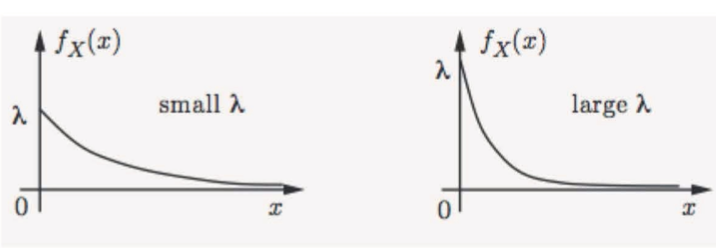
\includegraphics[width=0.5\textwidth]{L4_exp_pdf.png}
\end{frame}

%%%%%%%%%%%%%%%%%%%%%%%%%%%%%%%%%%%%%%%%%%%%%%%%%%%%%%
\begin{frame}{Geometric vs. Exponential (2)}

\plitemsep 0.1in
\bci

\item \redf{`slot'} is one unit time, e.g., 1 hour, 30 mins, 1 min, 10 sec, etc.

\item<2-> Continuous system = Discrete system with
\bci
\item \bluef{infinitely many slots} whose duration is \bluef{infinitely small}.
\item success probability $p$ over one slot \bluef{decreases to 0} in the limit
\eci

\item<3-> Given $X^{exp} \sim \exp(\lambda)$, let us construct a geometric RV $X^{geo}_\delta$

\bci
\item<4-> Set the length of a slot to be $\delta,$ which is a parameter.
\item<5-> Set the success probability $p_\delta$ over a slot to be $p_\delta = 1 - e^{-\lambda \delta}$ (this looks magical, whose secrete will be uncovered soon)
\item<6-> $\cprob{X^{geo}_\delta \leq n} = 1-(1-p_\delta)^n = 1- e^{-\lambda \delta n}$
\eci
\eci
\end{frame}

%%%%%%%%%%%%%%%%%%%%%%%%%%%%%%%%%%%%%%%%%%%%%%%%%%%%%%
\begin{frame}{Geometric vs. Exponential (3)}

\mypic{0.3}{L4_exp_geo.png}

\vspace{-0.5cm}
\plitemsep 0.07in
\bci

\item<2-> Note that $\cprob{X^{exp} \leq x} = 1- e^{-\lambda x}.$ Then, when $x = n\delta,$ $n=1, 2, \ldots$
$$
\cprob{X^{exp} \leq x} = 1- e^{-\lambda \delta n} = \onslide<3->{\cprob{X^{geo}_\delta \leq n} }
$$

\item<4-> If we choose sufficiently small $\delta$, the slot length $\downarrow$ and $p_\delta$ $\downarrow$
\mycolorbox{
$\cprob{X^{geo}_\delta \leq n}  \xrightarrow{\delta \rightarrow 0} \cprob{X^{exp} \leq x},$ $x = n \delta$
}
\eci

\end{frame}

% %%%%%%%%%%%%%%%%%%%%%%%%%%%%%%%%%%%%%%%%%%%%%%%%%%%%%%
% \begin{frame}{Modeling Waiting Time? A Discrete Twin (3)}
%
% \myvartwocols{0.7}{0.65}{0.33}
% {
% For a given $x>0,$
%
% \plitemsep 0.05in
% \bci
% \item<2-> Define $\delta = \frac{x}{n}$ (a slot length in the $n$-th system)
%
% \item<3-> Remember
% \aleq{
% F_{exp}(x) &= 1- \elambdax \cr
% F^n_{geo}(n) &= 1- (1-p_n)^n
% }
% \item<4-> Choose $p_n = 1-e^{-\lambda \delta} = 1-e^{-\lambda \frac{x}{n}}.$
%
% \item<5-> As $n \rightarrow \infty,$ the slot length $\delta \rightarrow 0$ thus $p_n \rightarrow 0$
%
% \item<5-> The CDF values of exponential and $n$-th geometric rvs become equal whenever $x =\delta, 2\delta, 3\delta, \ldots,$ i.e.,
% \aleq{
% F_{exp}(n\delta) = F^n_{geo}(n), \quad n=1, 2, \ldots
% }
%
% \eci
% }
% {
% % \raggedleft
% 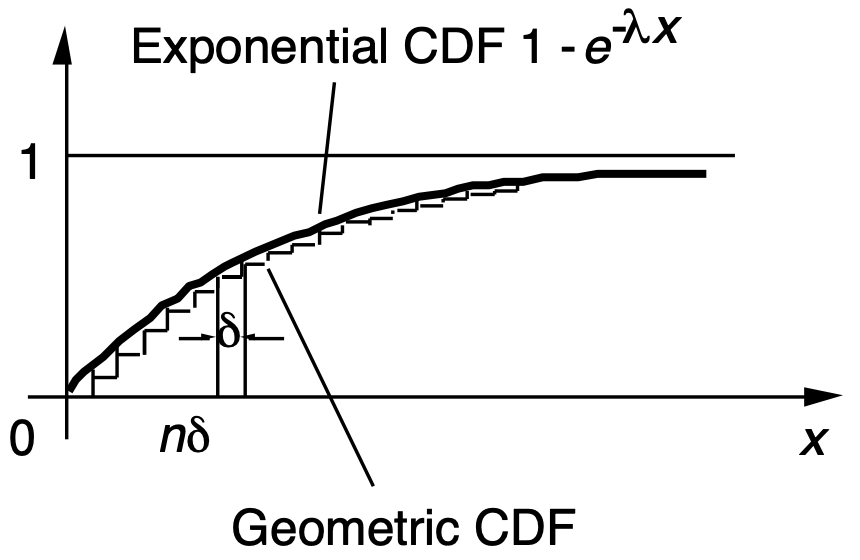
\includegraphics[width=0.95\textwidth]{L4_exp_geo.png}
% \small
% \bci
% \item<6-> As $n$ grows, the number of slots grows, but the success probability over one slot decreases, so that everything is balanced up.
% \item<7-> As $n$ grows, $F^n_{geo}(n)$ approaches $F_{exp}(n\delta).$
% \eci
% }
% \end{frame}

% %%%%%%%%%%%%%%%%%%%%%%%%%%%%%%%%%%%%%%%%%%%%%%%%%%%%%%
\section{L4(4)}
\begin{frame}{Roadmap}

\plitemsep 0.1in
\bce[(1)]
\item \grayf{Continuous Random Variable and PDF (Probability Density Function)}

\item \grayf{CDF (Cumulative Distribution Function)}

\item \grayf{Exponential RVs}

\item \redf{Gaussian (Normal) RVs}

\item \grayf{Continuous RVs: Joint, Conditioning, and Independence

\item Bayes' rule for RVs}

\ece
\end{frame}



%%%%%%%%%%%%%%%%%%%%%%%%%%%%%%%%%%%%%%%%%%%%%%%%%%%%%%
\begin{frame}{Normal: PDF, Expectation, Variance}

\mytwocols{0.4}
{
\plitemsep 0.01in
\bci
\item<1-> \orangef{Standard} Normal $\set{N}(0,1)$
\aleq{
\fx & = \frac{1}{\sqrt{2\pi}} e^{-x^2/2}
}
\item<1-> $\expect{X} = 0$

\item<1-> $\var{X} = 1$
\eci
}
{
\plitemsep 0.01in
\bci
\item<2-> General Normal $\set{N}(\mu, \sigma^2)$
\aleq{
\fx & = \frac{1}{\sigma\sqrt{2\pi}} e^{-(x-\mu)^2/2\sigma^2}
}

\item<2-> $\expect{X} = \mu$

\item<2-> $\var{X} = \sigma^2$

\eci
}

\vspace{-1cm}
\onslide<2->{\mypic{0.8}{L4_normal_ex.png}}
\vspace{-1cm}
\end{frame}

%%%%%%%%%%%%%%%%%%%%%%%%%%%%%%%%%%%%%%%%%%%%%%%%%%%%%%
\begin{frame}{Check: PDF, Expectation, Variance}

\plitemsep 0.07in
\bci
\item PDF's normalization property: $\displaystyle \frac{1}{\sigma\sqrt{2\pi}} \int_{-\infty}^\infty e^{-(x-\mu)^2/2\sigma^2} dx = 1$
\bci
\item<2-> A little bit boring :-). See Problem 14 at pp 189.
\eci

\item<3-> Expectation
\bci
\item $\fx$ is symmetric in terms of $x = \mu.$ Thus, we should have $\cexpect{X} = \mu.$
\eci

\item<4-> Variance
\aleq{
\cvar{X} &= \frac{1}{\sigma\sqrt{2\pi}} \int_{-\infty}^\infty (x - \mu)^2 e^{-(x-\mu)^2/2\sigma^2} dx
 \stackrel{\bluef{y=\frac{x-\mu}{\sigma}}}{=} \frac{\sigma^2}{\sqrt{2\pi}} \int_{-\infty}^\infty y^2 e^{-y^2/2} dy \cr
&= \frac{\sigma^2}{\sqrt{2\pi}}(-y e^{-y^2/2})\biggr \rvert_{-\infty}^\infty + \frac{\sigma^2}{\sqrt{2\pi}} \int_{-\infty}^\infty e^{-y^2/2} dy = \frac{\sigma^2}{\sqrt{2\pi}}\int_{-\infty}^\infty e^{-y^2/2} dy = \sigma^2
}

\mycolorbox{
\magenf{$\int u dv = u v - \int v du$:} \redf{$u=y$} and \bluef{$dv = y e^{-y^2/2}$} $\rightarrow$ \redf{$du = dy$} and \bluef{$v = -e^{-y^2/2}$}
}
\eci

\end{frame}

%%%%%%%%%%%%%%%%%%%%%%%%%%%%%%%%%%%%%%%%%%%%%%%%%%%%%%
\begin{frame}{Normality: Preserved under Linear Transformation}

\plitemsep 0.1in
\bci
\item<2-> Linear transformation preserves normality (we will verify this in Lecture 5)

\mycolorbox
{
If $X \sim  \set{N}(\mu, \sigma^2) $, then for $a \neq 0$ and $b,$ $Y = aX +b \sim \set{N}(a\mu +b,a^2 \sigma^2).$
}

\item<3-> Thus, every normal rv can be \redblank{4}{standardized}:

If $X \sim  \set{N}(\mu, \sigma^2)$, then
\redblank{4}{$Y = \frac{X-\mu}{\sigma}$} $\sim \set{N}(0,1)$

\item<5-> Thus, we can make the \redf{table} which records the following CDF values:
\aleq{
\Phi(y) = \cprob{Y \le y} = \cprob{Y < y} = \frac{1}{\sqrt{2\pi}} \int_{-\infty}^y e^{-t^2/2} dt
}


\eci
\end{frame}

%%%%%%%%%%%%%%%%%%%%%%%%%%%%%%%%%%%%%%%%%%%%%%%%%%%%%%
\begin{frame}{Example}

\medskip

\mytwocols{0.7}
{
\plitemsep 0.1in
\bci
\item<1-> Annual snowfall $X$ is modeled as $\set{N}(60,20^2).$ What is the probability that this year's snowfall is at least 80 inches?

\item<2-> $Y = \frac{X-60}{20}.$
\onslide<3->{
\aleq{
\cprob{X \ge 80} &= \cprob{Y \ge \frac{80-60}{20}} \cr
&= \cprob{Y \ge 1} = 1 -
\Phi(1) \cr
&= 1- 0.8413 = 0.1587
}
}
\eci
}
{
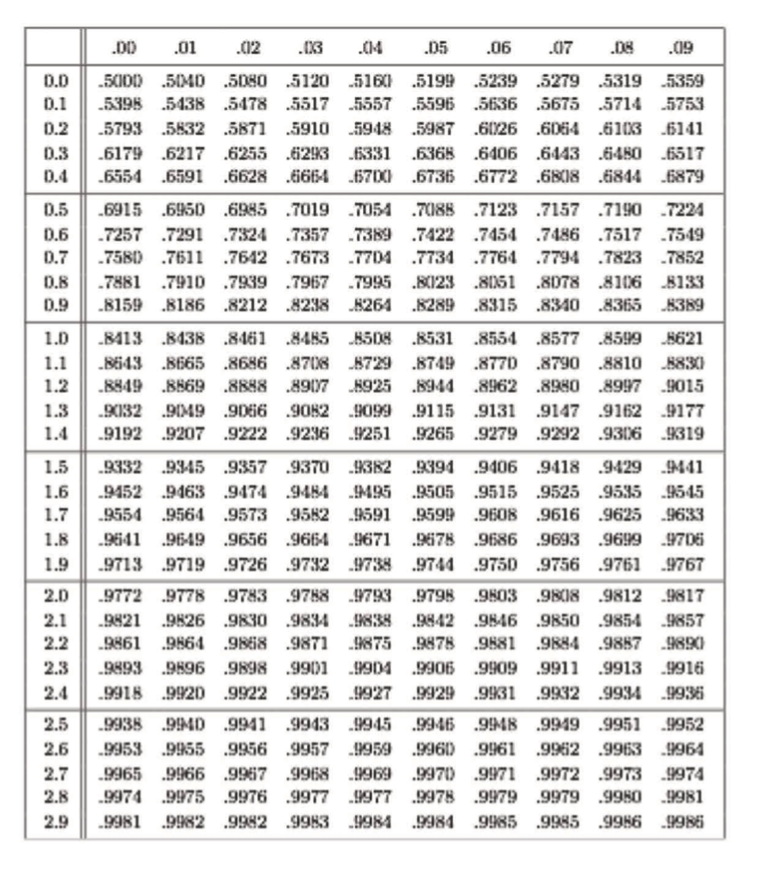
\includegraphics[width=0.8\textwidth]{L4_normal_table.png}
}
\end{frame}



%%%%%%%%%%%%%%%%%%%%%%%%%%%%%%%%%%%%%%%%%%%%%%%%%%%%%%
\begin{frame}{Normal RVs: Why Important?}
\footnotetext{Central limit theorem: 중심극한정리}

\plitemsep 0.15in
\bci
\item Central limit theorem

\bci
\item  One of the most remarkable findings in the probability theory
\item  Sum of \redf{any} random variables $\approx$ Normal random variable
\eci

\item Modeling aggregate noise with many small, independent noise terms

\item Convenient analytical properties, allowing closed forms in many cases

\item Highly popular in communication and machine learning areas
\eci
\end{frame}


% %%%%%%%%%%%%%%%%%%%%%%%%%%%%%%%%%%%%%%%%%%%%%%%%%%%%%%
\section{L4(5)}
\begin{frame}{Roadmap}

\plitemsep 0.1in
\bce[(1)]
\item \grayf{Continuous Random Variable and PDF (Probability Density Function)}

\item \grayf{CDF (Cumulative Distribution Function)}

\item \grayf{Exponential RVs}

\item \grayf{Gaussian (Normal) RVs}

\item \redf{Continuous RVs: Joint, Conditioning, and Independence}

\item \grayf{Bayes' rule for RVs}

\ece
\end{frame}


%%%%%%%%%%%%%%%%%%%%%%%%%%%%%%%%%%%%%%%%%%%%%%%%%%%%%%
\begin{frame}{Continuous: Joint PDF and CDF (1)}

\mycolorbox
{
Two continuous rvs are \redblank{2}{jointly continuous} if a non-negative function $\fxy$ (called joint PDF) satisfies: for \redf{every subset} $B$ of the two dimensional plane,
$$
\cprob{(X,Y) \in B} = \iint_{(x,y) \in B} \fxy dx dy,
$$
\vspace{-0.3cm}
}

\plitemsep 0.1in
\bce
\item<3-> The joint PDF is used to calculate probabilities
$$\bprob{(X,Y) \in B} = \iint_{(x,y) \in B} \fxy dx dy$$

Our particular interest: $B = \{(x,y) \mid a \le x \le b, c \le y \le d \}$
\ece

\end{frame}

%%%%%%%%%%%%%%%%%%%%%%%%%%%%%%%%%%%%%%%%%%%%%%%%%%%%%%
\begin{frame}{Continuous: Joint PDF and CDF (2)}

\plitemsep 0.1in
\bce
\item<1->[2.] The \redf{marginal} PDFs of $X$ and $Y$ are from the joint PDF as:
$$
\fx = \int_{-\infty}^\infty \fxy dy, \quad \fy = \int_{-\infty}^\infty \fxy dx
$$

\item<2->[3.] The \redf{joint CDF} is defined by $\Fxy = \cprob{X \le x, Y \le y},$ and determines the joint PDF as:
$$
\fxy = \frac{\partial^2 F_{x,y}}{\partial x \partial y} (x,y)
$$

\item<3->[4.] A function $g(X,Y)$ of $X$ and $Y$ defines a new random variable, and
$$
\expect{g(X,Y)} = \int_{-\infty}^\infty \int_{-\infty}^\infty g(x,y) \fxy dx dy
$$
\ece

\end{frame}

%%%%%%%%%%%%%%%%%%%%%%%%%%%%%%%%%%%%%%%%%%%%%%%%%%%%%%
\begin{frame}{Continuous:  Conditional PDF given an event}

\mytwocols{0.5}
{
* Conditional PDF, given an event $A$

\medskip

\plitemsep 0.15in
\bci
\item<2-> $\fx \cdot \delta \approx \cprob{x \le X \le x+\delta}$
$\redf{\fxA} \cdot \delta \approx \cprob{x \le X \le x+\delta | A}$

\item<3-> $\cprob{X \in B} = \int_B \fx dx$
$\cprob{X \in B | A} = \int_B \fxA dx$



\item<4-> $\int \fxA dx= 1$
\eci
}
{
* Conditional PDF, given $\{X \in C \}$

\medskip

\onslide<5->{
\aleq{
\redf{f_{X|\{X \in C\}}(x)} \cdot \delta \approx \cprob{x \le X \le x+ \delta | X \in C}
}
\aleq{
f_{X|\{X \in C\}}(x) =
\begin{cases}
0, & \text{if} \quad x \notin C \cr
\frac{\fx}{\cprob{X \in C}}, &\text{if} \quad x \in C
\end{cases}
}}

\onslide<6->{\redf{(Q)} In the discrete, we consider the event $\{X = x\}$, not $\{X \in B\}.$ Why?}

}

\redf{Notation:} $A$ is an event, but $B$ and $C$ is a subset that includes the possible values which can be taken by the rv $X.$ Sorry for the confusion, if any.


\end{frame}

%%%%%%%%%%%%%%%%%%%%%%%%%%%%%%%%%%%%%%%%%%%%%%%%%%%%%%
\begin{frame}{Continuous:  Conditional Expectation}

\mytwocols{0.75}
{
\plitemsep 0.15in

\onslide<3->{$A = \{\frac{a+b}{2} \le X \le b \}$}

%\smallskip

\vspace{-0.3cm}
\onslide<3->{\mypic{0.65}{L4_cond_ex1.png}}
\vspace{-0.5cm}
\only<3>{\mypic{0.65}{L4_cond_ex2.png}}
\vspace{-0.5cm}
\only<4->{\mypic{0.65}{L4_cond_ex3.png}}

}
{
\bci
\item<1-> $\expect{X} = \int x\fx dx$
$\expect{X | A} = \int x\fxA dx$

\item<2-> $\expect{g(X)} = \int g(x)\fx dx$
$\expect{g(X) | A} = \int g(x)\fxA dx$
\eci

\onslide<3->{
\aleq{
\expect{X|A} = \onslide<4->{\int_{(a+b)/2}^b x \frac{2}{b-a} dx = \frac{a}{4} + \frac{3b}{4}}
}
}
\onslide<3->{
\aleq{
\expect{X^2|A} = \onslide<4->{\int_{(a+b)/2}^b x^2 \frac{2}{b-a} dx =}
}}
}
\end{frame}

%%%%%%%%%%%%%%%%%%%%%%%%%%%%%%%%%%%%%%%%%%%%%%%%%%%%%%
\begin{frame}{Exponential RV: Memoryless}

\plitemsep 0.1in
\bci
\item<1-> \redf{Remember:} Exponential rv is a continuous counterpart of geometric rv.
\item<2-> Thus, expected to be memoryless. Remember the definition?

\onslide<3->{
\bigskip
\bluef{Definition.} A random variable $X$ is called memoryless if, for any $n,m \ge 0,$
\redblank{4}{$\cprob{X > n+m | X > m} = \cprob{X > n}$}
}

\item<4-> \redf{Proof.} Note that the exponential rv's CCDF $\cprob{X > x} = \elambdax.$
\onslide<5->{
Then,
\aleq{
\cprob{X > n+m | X > m} = \frac{\cprob{X > n+m}}{\cprob{X > m}} = \frac{e^{-\lambda(n+m)}}{e^{-\lambda m}} = e^{-\lambda n} = \cprob{X > n}
}
}

\eci

\end{frame}

%%%%%%%%%%%%%%%%%%%%%%%%%%%%%%%%%%%%%%%%%%%%%%%%%%%%%%
\begin{frame}{Total Probability/Expectation Theorem}

Partition of $\Omega$ into $A_1,A_2,A_3, \ldots$

\medskip

\mytwocols{0.7}
{
\small
* Discrete case
\medskip

\begin{block}<2->{Total Probability Theorem}
\aleq{
 \px &= \sum_{i} \cprob{A_i} \cprob{X=x | A_i} \cr
 &= \sum_{i} \cprob{A_i} p_{X|A_i}(x)
}
 \end{block}

\begin{block}<2->{Total Expectation Theorem}
\aleq{
 \expect{X} = \sum_{i} \cprob{A_i} \expect{X | A_i}
}
\end{block}
}
{
\small
* Continuous case
\medskip


\begin{block}<3->{Total Probability Theorem}
\aleq{
 \redf{\fx} = \sum_{i} \cprob{A_i} \redf{f_{X|A_i}(x)}
}
 \end{block}

\begin{block}<4->{Total Expectation Theorem}
\aleq{
 \expect{X} = \sum_{i} \cprob{A_i} \expect{X | A_i}
}
\end{block}
}

\end{frame}

%%%%%%%%%%%%%%%%%%%%%%%%%%%%%%%%%%%%%%%%%%%%%%%%%%%%%%
\begin{frame}{Example: Train Arrival }

\mytwocols{0.8}
{

\bigskip




\plitemsep 0.1in
\bci
\item<1-> The train's arrival every quarter hour (0, 15min, 30min, 45min).

\item<1-> Your arrival $\sim$ \set{U}(7:10, 7:30) am.

\item<2-> What is the PDF of waiting time for the first train?

\item<3-> $X:$ your arrival time, $Y:$ waiting time.

\item<4-> The value of $X$ makes a different waiting time. So, consider two events:

\medskip
$A = \{\text{7:10} \leq X \leq \text{7:15} \}$

\medskip
$B = \{\text{7:15} \leq X \leq \text{7:30} \}$

%\item Then, using the total probability theorem,
\eci
}
{
\small
\vspace{-0.3cm}
\mypic{0.85}{L4_total_prob_ex.png}
\vspace{-0.3cm}
\onslide<5>{\hfill \lecturemark{VIDEO PAUSE}}
\aleq{
\onslide<5->{&\fy  = \cprob{A} \fyA + \cprob{B} f_{Y|B}(y)} \cr
&\onslide<6->{\fy = {1 \over 4} {1 \over 5} +{3 \over 4} {1 \over 15} = {1 \over 10},} \quad \onslide<5->{\text{for } 0 \le y \le 5} \cr
&\onslide<7->{\fy = {1 \over 4} 0 +{3 \over 4} {1 \over 15} = {1 \over 20},} \quad \onslide<5->{\text{for } 5 < y \le 15}
}
}

\end{frame}

%%%%%%%%%%%%%%%%%%%%%%%%%%%%%%%%%%%%%%%%%%%%%%%%%%%%%%
\begin{frame}{Continuous:  Conditional PDF given a RV}

\mytwocols{0.8}
{
\medskip
\small
\plitemsep 0.1in
\bci

\item $\pxcy = \frac{\pxy}{\py}$

\item<2-> Similarly, for $\fy >0,$
$$
\fxcy = \frac{\fxy}{\fy}
$$

\item<3-> Remember: For a fixed event $A,$ $\cprob{\cdot | A}$ is a legitimate probability law.

\item<4-> Similarly, For a fixed $y,$ $\fxcy$ is a legitimate PDF, since
$$
\int_{-\infty}^\infty \fxcy \redf{dx} = \frac{\int_{-\infty}^\infty \fxy dx}{\fy} = 1
$$
\eci
}
{
\medskip
\small
\plitemsep 0.01in
\bci

\item<5-> \redf{Multiplication rule.}
\aleq{
\fxy &= \fy \cdot \fxcy = \fx \fycx
}

\item<6-> \redf{Total prob./exp. theorem.}
\aleq{
\fx &= \int_{-\infty}^\infty \fy \fxcy dy \cr
\expect{X | Y=y} &= \int_{-\infty}^\infty x \fxcy dx \cr
\expect{X} &= \int_{-\infty}^\infty \fy \expect{X | Y=y} dy
}

\item<7-> \redf{Independence}
\aleq{
\fxy = \fx \fy, \quad \text{for all $x$ and $y$}
}
\eci
}
\end{frame}

%%%%%%%%%%%%%%%%%%%%%%%%%%%%%%%%%%%%%%%%%%%%%%%%%%%%%%
\begin{frame}{Example: Stick-breaking (1)}

\noindent\bluef{(Prob 21 at pp. 191)}

\footnotetext{$\set{U}[a,b]$: continuous uniform random variable over the interval $[a,b]$}
\mytwocols{0.7}
{
\small
\plitemsep 0.1in
\bci

\item<1-> Break a stick of length $l$ twice

- first break at $Y \sim \set{U}[0,l]$

- second break at $X \sim \set{U}[0,Y]$

\item<2->[\redf{(a)}] joint PDF $\fxy$?
\aleq
{
\fy &= \frac{1}{l}, \quad 0 \le y \le 1\cr
\fxcy & = \frac{1}{y}, \quad 0 \le x \le y
}
Using $\fxy = \fy \fxcy,$
\aleq{
\fxy =
\begin{cases}
\frac{1}{l}\cdot\frac{1}{y}, & 0 \le x \le y \le l,\cr
0, & \text{otherwise}
\end{cases}
}
% \item<2-> \redf{(Q)} What is $\expect{Y}$?
%
% \item<3-> Since $Y$ depends on $X,$ the total expectation theorem seems useful.
% $$
% \expect{Y} = \int_{-\infty}^\infty \fx \expect{Y| X=x} dx
% $$

\eci
}
{
%\medskip
%\small
\small
\plitemsep 0.1in
\bci

\item<3->[\redf{(b)}] marginal PDF $\fx$?
\aleq
{
\fx &= \int \fxy dy = \int_{x}^l \frac{1}{ly} dy \cr
& = \frac{1}{l} \ln(l/x), \quad 0 \le x \le l
}


% \item<4-> Using the TET,
% \aleq{
% \expect{Y} &= \int_{0}^l \frac{1}{l} \expect{Y| X=x} dx\cr
% &= \int_{0}^l \frac{1}{l} \frac{x}{2} dx = \frac{l}{4}
% }
%
% \item<5-> $\fx$ and $\fycx$ seems easy to compute. Thus,
% \aleq{
% \fxy &= \fx \fycx = {1 \over l} \cdot {1 \over x}
% }
% You can do many other things with the joint PDF.
\eci
}

\end{frame}

%%%%%%%%%%%%%%%%%%%%%%%%%%%%%%%%%%%%%%%%%%%%%%%%%%%%%%
\begin{frame}{Example: Stick-breaking (2)}

\mytwocols{0.75}
{
\small
\plitemsep 0.1in
\bci

\item<1->[\redf{(c)}] Evaluate $\cexpect{X}$, using $\fx$
\aleq
{
\onslide<2->{
\cexpect{X} &= \int_{0}^l x \fx dx = \int_{0}^l \frac{x}{l} \ln(l/x) dx \cr
& = \frac{l}{4}
}
}


\item<1->[\redf{(d)}] Evaluate $\cexpect{X}$, using $X = Y\cdot (X/Y)$

\medskip

If $Y \indep X/Y,$ it becomes easy, but true?

\onslide<3->{
Yes, because whatever $Y$ is,
the fraction $X/Y$ does not depend on it.
\aleq{
\cexpect{X} = \cexpect{Y} \cexpect{X/Y} = \frac{l}{2} \cdot \frac{1}{2} = \frac{l}{4}
}
}


\eci
}
{
\small
\plitemsep 0.1in
\bci

\item<1->[\redf{(e)}] Evaluate $\cexpect{X}$, using TET
\aleq
{
\onslide<4->{0
\expect{X} &= \int_{-\infty}^\infty \fy \expect{X| Y=y} dy \cr
&= \int_{0}^l \frac{1}{l} \expect{X| Y=y} dy
= \int_{0}^l \frac{1}{l} \frac{y}{2} dy = \frac{l}{4}
}
}


\item<5-> \msg There are many ways to rearch our goal. Of crucial importance is how to find the best way!
\eci
}



\end{frame}



% %%%%%%%%%%%%%%%%%%%%%%%%%%%%%%%%%%%%%%%%%%%%%%%%%%%%%%
\section{L4(6)}
\begin{frame}{Roadmap}

\plitemsep 0.1in
\bce[(1)]
\item \grayf{Continuous Random Variable and PDF (Probability Density Function)}

\item \grayf{CDF (Cumulative Distribution Function)}

\item \grayf{Exponential RVs}

\item \grayf{Gaussian (Normal) RVs}

\item \grayf{Continuous RVs: Joint, Conditioning, and Independence}

\item \redf{Bayes' rule for RVs}

\ece
\end{frame}


%%%%%%%%%%%%%%%%%%%%%%%%%%%%%%%%%%%%%%%%%%%%%%%%%%%%%%
\begin{frame}{Bayes Rule for Continuous}

\plitemsep 0.1in


\mycolorbox{
\bci
\item<1-> $X$: state/cause/original value $\rightarrow$ $Y$: result/resulting action/noisy measurement

\item<1-> Given: $\cprob{X}$ and $\cprob{Y | X}$ (cause $\rightarrow$ result)

\item<1-> Inference: $\cprob{X | Y}$?
\eci
}
 \medskip
 \mytwocols{0.35}
 {
\onslide<2->{
\aleq{
\pxy & = \px \pycx \cr
     & = \py \pxcy \cr
\redf{\pxcy} & = \frac{\px \pycx}{\py}\cr
\py &= \sum_{x'} p_X(x')p_{Y|X}(y|x')
}
 }}
{

\aleq{
\onslide<2->{
\fxy & = \fx \fycx \cr
     & = \fy \fxcy \cr
\redf{\fxcy} & = \frac{\fx \fycx}{\fy}\cr
\fy &= \int f_X(x')f_{Y|X}(y|x') dx'
}
}
}

\end{frame}



%%%%%%%%%%%%%%%%%%%%%%%%%%%%%%%%%%%%%%%%%%%%%%%%%%%%%%
\begin{frame}{Example}

\plitemsep 0.1in

\bci
\item<1-> A light bulb $Y \sim \exp(\lambda).$ However, there are some quality control problems.
So, the parameter $\lambda$ of $Y$ is actually a random variable, denoted by $\Lambda$, which is $\Lambda \sim \set{U}[1,3/2].$ We test a light bulb and record its lifetime.

\item<2-> \question What can we say about the underlying paramter $\lambda$? In other words, what is $f_{\Lambda | Y}(\lambda|y)$?

\item<3-> $f_{\Lambda}(\lambda) = 2$ for $1 \le \lambda \le 3/2$ and $f_{Y | \Lambda}  (y | \lambda) = $ pdf of $\exp(\lambda).$ Then, the inference about the parameter given the lifetime of a light bulb is:
\onslide<4->
{
$$
f_{\Lambda | Y}(\lambda|y) = \frac{f_\Lambda(\lambda)f_{Y | \Lambda}  (y | \lambda) }{\int_{-\infty}^\infty f_\Lambda(t) f_{Y | \Lambda}(y | t) dt}
$$
}
\eci

\end{frame}

%%%%%%%%%%%%%%%%%%%%%%%%%%%%%%%%%%%%%%%%%%%%%%%%%%%%%%
\begin{frame}{Using Bayes Rule for Parameter Learning}

\mycolorbox{
\bci
\item<1-> $X$: \bluef{\bf parameter} $\rightarrow$ $Y$: result of \redf{\bf my model}

\item<1-> Given: $\cprob{X}$ and $\cprob{Y | X}$ (parameter $\rightarrow$ model)

\item<1-> Inference: $\cprob{X | Y}$? Probabilistic feature of the parameter given the result of the model?
\eci
}


\plitemsep 0.07in

\exam

\bce
\item<2-> Light bulb's lifetime $Y \sim \exp(\bluef{\lambda}).$ Given the lifetime \redf{$y$}, the modified belief about \bluef{$\lambda$}?

\item<3-> Romeo and Juliet start dating, but Romeo will be late by a random variable $Y \sim \set{U}[0,\bluef{\theta}].$ Given the time of being late \redf{$y$}, the modified belief about \bluef{$\theta$}?
\ece

\end{frame}


%%%%%%%%%%%%%%%%%%%%%%%%%%%%%%%%%%%%%%%%%%%%%%%%%%%%%%
\begin{frame}{Bayes Rule for Mixed Case}

\onslide<1->{$K$: discrete, $Y$: continuous}

\bigskip

\plitemsep 0.1in
\mytwocols{0.5}
{

\bci
\item<2-> Inference of $K$ given $Y$
\aleq{
\onslide<3->{
\redf{p_{K|Y}(k|y)} &= \frac{\redf{p_{K}(k)} \bluef{f_{Y|K}(y|k)}}{\bluef{\fy}}\cr
\bluef{\fy} &= \sum_{k'} \redf{p_{K}(k')} \bluef{f_{Y|K}(y|k')}
}
}
\item<4-> $f_{Y|K}(y|k) = f_{Y | A}(y),$ where $A = \{K=k\}$
\eci

}
{
\bci



\item<2-> Inference of $Y$ given $K$
\aleq{
\onslide<5->{
\bluef{f_{Y|K}(y|k)} &= \frac{\bluef{\fy} \redf{p_{K|Y}(k|y)}}{\redf{p_{K}(k)}} \cr
\redf{p_{K}(k)} &= \int \bluef{f_{Y}(y')} \redf{p_{K|Y}(k|y')} dy'
}}
\item<6-> Wait! $p_{K|Y}(k|y)$? Well-defined?
\aleq{
p_{K|Y}(k|y) = \frac{\cprob{K=k, Y=y}}{\cprob{Y=y}} = \frac{0}{0}
}

\eci
}

\end{frame}

%%%%%%%%%%%%%%%%%%%%%%%%%%%%%%%%%%%%%%%%%%%%%%%%%%%%%%
\begin{frame}{$p_{K|Y}(k|y)$?}


\plitemsep 0.1in

\bci
\item For small $\delta$ (in other words, taking the limit as $\delta \rightarrow 0$).

\medskip
Let $A = \{K=k\}.$

\bigskip
\aleq{
\redf{p_{K|Y}(k|y)} & \approx \cprob{ A | y \le Y \le y+ \delta}\cr
&= \frac{\cprob{A} \cprob{y \le Y \le y+ \delta | A}}{\cprob{y \le Y \le y+ \delta}}\cr
&\approx \frac{\cprob{A} f_{Y|A}(y)\delta}{\fy \delta}\cr
&= \redf{\frac{\cprob{A} f_{Y|A}(y)}{\fy }}
}


\eci

\end{frame}

%%%%%%%%%%%%%%%%%%%%%%%%%%%%%%%%%%%%%%%%%%%%%%%%%%%%%%
\begin{frame}{Example: Signal Detection (1)}


\mycolorbox{
Inference of discrete $K$ given continuous $Y$:
\aleq{
\redf{p_{K|Y}(k|y)} = \frac{\redf{p_{K}(k)} \bluef{f_{Y|K}(y|k)}}{\bluef{\fy}}, \quad \bluef{\fy} &= \sum_{k'} \redf{p_{K}(k')} \bluef{f_{Y|K}(y|k')}
}}

\plitemsep 0.01in
\bci

\item<2-> $K$: -1, +1, original signal, equally likely. $p_{K}(1) = 1/2, p_{K}(-1) = 1/2.$
\item<3-> $Y$: measured signal with Gaussian noise, $Y= K+W,$ $W \sim \set{N}(0,1)$

\medskip
\item<4-> Your received signal = 0.7. What's your guess about the original signal? \onslide<6->{\redf{+1}}
\item<5-> Your received signal = -0.2. What's your guess about the original signal? \onslide<6->{\redf{-1}}



\medskip
\item<6-> Your intuition: If positive received signal, +1. If negative received signal, -1. How can we mathematically verify this?
\eci
\end{frame}

%%%%%%%%%%%%%%%%%%%%%%%%%%%%%%%%%%%%%%%%%%%%%%%%%%%%%%
\begin{frame}{Example: Signal Detection (2)}

\plitemsep 0.01in
\bci

\item<1-> $Y|\{K=1\} \sim \set{N}(1,1)$ and $Y|\{K=-1\} \sim \set{N}(-1,1).$ \\
(Remind: linear transformation preserves normality.)
\aleq{
\onslide<2->{f_{Y|K}(y|k) &= \frac{1}{\sqrt{2 \pi}} e^{-\frac{1}{2}(y-k)^2}, \quad k=1, -1} \cr
\onslide<3->{\fy &= \frac{1}{2} \frac{1}{\sqrt{2 \pi}} e^{-\frac{1}{2}(y+1)^2} +
\frac{1}{2} \frac{1}{\sqrt{2 \pi}} e^{-\frac{1}{2}(y-1)^2} \qquad \qquad \text{(from TPT)}}
}

\item<4-> Probability that $K=1$, given $Y=y$? After some algebra,

\mytwocols{0.3}
{
$$
p_{K|Y}(1|y) = \frac{1}{1+ e^{-2y}}
$$
\vspace{-0.3cm}
\bci
\item<6->  If $y >0,$ the inference probability for $K=1$ exceeds $\frac{1}{2}$. So, original signal = 1.
\item<7->  Similarly, compute $p_{K|Y}(-1|y)$ and then do the inference
\eci


}
{
\centering
\onslide<5->{\mypic{0.8}{L4_sig_detection.png}}
}

\eci

\end{frame}

\begin{frame}{}
\vspace{2cm}
\LARGE Questions?

\end{frame}

\begin{frame}{Review Questions}

\bce[1)]
\item What is PDF  and CDF?

\item Why do we need CDF?

\item What are joint/marginal/conditional PDFs?

\item Explain memorylessness of exponential random variables.

\item Explain the version of Bayes' rule for continuous and mixed random variables.

\ece

\end{frame}

\end{document}
